%%%%%%%%%%%%%%%%%%%%%%%%%%%%%%%%%%%%%%%%%
%
% CMPT 435
% Lab Zero
%
%%%%%%%%%%%%%%%%%%%%%%%%%%%%%%%%%%%%%%%%%

%%%%%%%%%%%%%%%%%%%%%%%%%%%%%%%%%%%%%%%%%
% Short Sectioned Assignment
% LaTeX Template
% Version 1.0 (5/5/12)
%
% This template has been downloaded from: http://www.LaTeXTemplates.com
% Original author: % Frits Wenneker (http://www.howtotex.com)
% License: CC BY-NC-SA 3.0 (http://creativecommons.org/licenses/by-nc-sa/3.0/)
% Modified by Alan G. Labouseur  - alan@labouseur.com
%
%%%%%%%%%%%%%%%%%%%%%%%%%%%%%%%%%%%%%%%%%

%----------------------------------------------------------------------------------------
%	PACKAGES AND OTHER DOCUMENT CONFIGURATIONS
%----------------------------------------------------------------------------------------

\documentclass[letterpaper, 10pt]{article} 

\usepackage[english]{babel} % English language/hyphenation
\usepackage{graphicx}
\usepackage{xcolor}
\graphicspath{ {./images/} }
\usepackage[lined,linesnumbered,commentsnumbered]{algorithm2e}
\usepackage{listings}
\usepackage{flafter} 


% Lstlistings configuration
\definecolor{codegreen}{rgb}{0,0.6,0}
\definecolor{codegray}{rgb}{0.5,0.5,0.5}
\definecolor{codepurple}{rgb}{0.58,0,0.82}
\definecolor{backcolour}{rgb}{0.95,0.95,0.92}

\lstdefinestyle{mystyle}{
    backgroundcolor=\color{backcolour},   
    commentstyle=\color{codegreen},
    keywordstyle=\color{magenta},
    numberstyle=\tiny\color{codegray},
    stringstyle=\color{codepurple},
    basicstyle=\ttfamily\footnotesize,
    breakatwhitespace=false,         
    breaklines=true,                 
    captionpos=b,                    
    keepspaces=true,                 
    numbers=left,                    
    numbersep=5pt,                  
    showspaces=false,                
    showstringspaces=false,
    showtabs=false,                  
    tabsize=2
}

\lstset{style=mystyle}
\lstset{language=Java}

\usepackage{fancyhdr} % Custom headers and footers
\pagestyle{fancyplain} % Makes all pages in the document conform to the custom headers and footers
\usepackage{lastpage}
\usepackage{wasysym}
\usepackage{url}

% Set up for minted package. It had some bugs so I decided to only keep lstlistings.
% \usepackage{minted}
% \makeatletter
% \newlength\minted@belowskip
% \define@key{minted@opt}{belowskip}[\@topsepadd]
% {\setlength{\minted@belowskip}{#1}}

% \def\minted@endparenv{%
%   \addpenalty\@endparpenalty\addvspace\minted@belowskip\@endpetrue}
% \def\FV@EndList{%
%   \FV@ListProcessLastLine
%   \FV@EndListFrame
%   \minted@endparenv
%   \endgroup
%   \@endpetrue}
% \makeatother
% \newminted{java}{linenos=true, belowskip=3cm}

\fancyhead{} % No page header - if you want one, create it in the same way as the footers below
\fancyfoot[L]{} % Empty left footer
\fancyfoot[C]{page \thepage\ of \pageref{LastPage}} % Page numbering for center footer
\fancyfoot[R]{}

\renewcommand{\headrulewidth}{0pt} % Remove header underlines
\renewcommand{\footrulewidth}{0pt} % Remove footer underlines
\setlength{\headheight}{13.6pt} % Customize the height of the header

%----------------------------------------------------------------------------------------
%	TITLE SECTION
%----------------------------------------------------------------------------------------

\newcommand{\horrule}[1]{\rule{\linewidth}{#1}} % Create horizontal rule command with 1 argument of height

\title{	
   \normalfont \normalsize 
   \textsc{CMPT 435 - Fall 2021 - Dr. Labouseur} \\[10pt] % Header stuff.
   \horrule{0.5pt} \\[0.25cm] 	% Top horizontal rule
   \huge Assignment Two -- Sorting Algorithms \\     	    % Assignment title
   \horrule{0.5pt} \\[0.25cm] 	% Bottom horizontal rule
}

\author{Augusto Gonzalez-Bonorino \\ \normalsize augusto.gonzalezbonorino1@marist.edu}

\date{\normalsize\today} 	% Today's date.

\begin{document}

\maketitle % Print the title

%----------------------------------------------------------------------------------------
%   CONTENT SECTION
%----------------------------------------------------------------------------------------

% - -- -  - -- -  - -- -  -

\section{Description of the program}
The program aims to implement, and compare, the following sorting algorithms: Insertion, Selection, Merge and Quick sort. In regards to my implementation in Java I have decided to define one MainGonzalezBonorino class which contains the functions necessary to read the input text document containing the Strings to sort and the functions needed to implement each algorithm.The characteristics and details of each algorithm will be explored in detail throughout this documentation


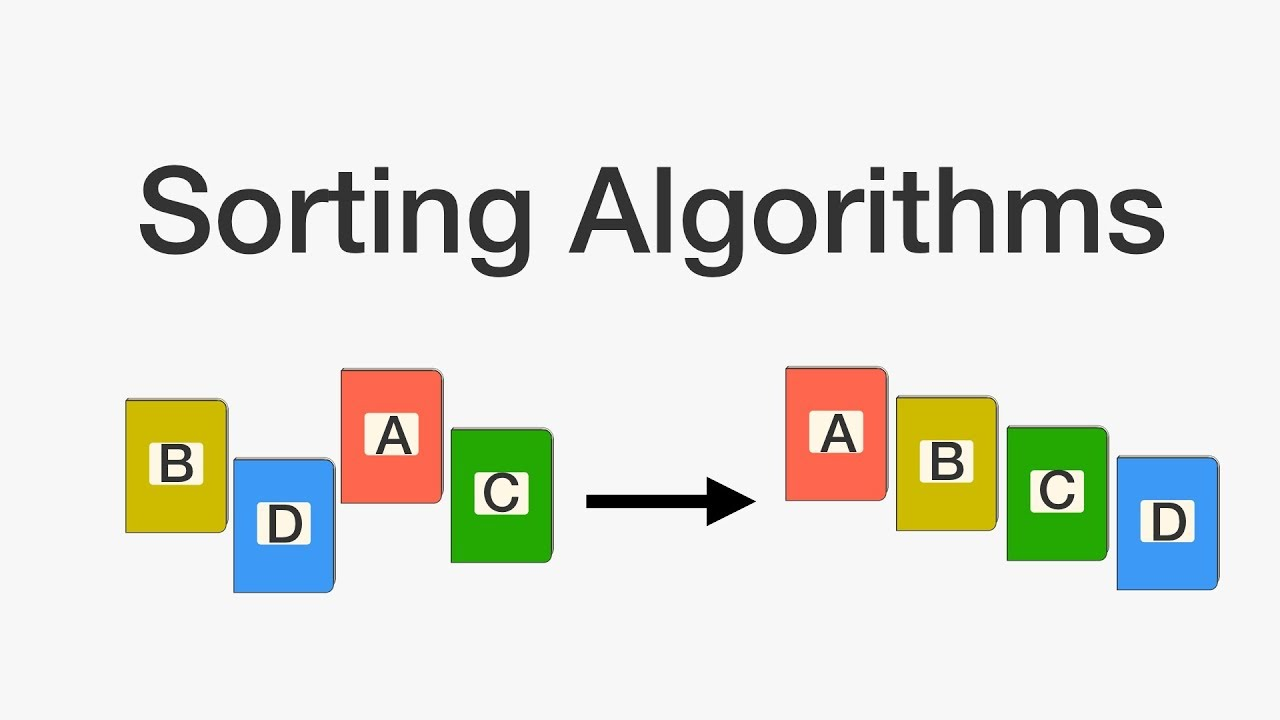
\includegraphics[scale=0.25]{images/sorting_algorithms.jpg}

\pagebreak
\section{Selection Sort}

Selection sort runs in $O(n^2)$ due to the nested for loops used to traverse the array and compare each element, it works as follows: It repeatedly finds the minimum element of an unsorted section of the array and places that element at the beginning, thereby maintaining two sub arrays (one sorted and one being sorted) until the whole array is traversed. In each iteration the minimum element is moved to the sorted sub array. 

\begin{lstlisting}
public static int selectionSort(String[] magicList) {
		
		knuthShuffle(magicList);
		int len = magicList.length;
		int numComparisons = 0;
		
		for (int i = 0; i < len - 1; i++) {
			
			int smallPos = i;
			
			for (int j = i + 1; j <= len - 1; j++) {
				
				if (magicList[j].compareToIgnoreCase(magicList[smallPos]) < 0 ) //compare strings
				{	
					smallPos = j;
				}
				numComparisons++;
						
			} // inner for loop
			
			// swap
			String temp = magicList[smallPos];
			magicList[smallPos] = magicList[i];
			magicList[i] = temp;
			
		} // outer for loop
		
		return numComparisons;
		
	} // selectionSort
\end{lstlisting}

The java implementation is fairly straightforward. First, to ensure the input array is shuffled, I implement a Knuth shuffle (a.k.a. the Fisher-Yates shuffle) which is commonly used to shuffle arrays. You will soon note that this function is used before implementing each sorting algorithm to make sure that we are not feeding the algorithm an already sorted array. Next, in the outer loop, we instantiate an integer called \textit{smallPos} to keep track of the index of the smallest element. Then, we use that index to loop over each String in the magicitems.txt file and compare them. If, after the comparison was made, one of them was smaller than the current smallest element then \textit{smallPos} is updated and the number of comparisons is incremented. Once we compared the elements, we swap them to create the sorted array. The algorithm repeats the aforementioned steps until the whole array is sorted.
\pagebreak
\section{Insertion Sort}

Insertion sort, like Selection, has a run time of $O(n^2)$. Nevertheless, this algorithm provides an improvement over Selection sort because it avoids looping over the array if a subset of it is already sorted, thereby saving us some precious resources. Therefore, while the worst-case scenario is $O(n^2)$ it is possible to reduce it to $O(n)$ if the array is already sorted. The algorithm divides the array into two sub arrays (sorted and unsorted). Then, values from the unsorted part are picked and placed at the correct position in the sorted part.

\begin{lstlisting}
public static int insertionSort(String[] magicList) {
		
		knuthShuffle(magicList);
		int len = magicList.length;
		int numComparisons = 0;
		
		for (int j = 1; j <= len - 2; j++) {
			
			String key = magicList[j];
			int i = j - 1;
			
			while ( (i >= 0) && ( magicList[i].compareToIgnoreCase(key) > 0) ) {
				
				magicList[i + 1] = magicList[i];
				i = i - 1;
				
				numComparisons++;
				
			} // while loop
			
			magicList[i + 1] = key;
			
		} // for loop
		
		return numComparisons;
		
	} // insertionSort
\end{lstlisting}

After shuffling the input array of Strings we assign the first element to a variable I have called \textit{key}. Then, we compare the current element \textit{key} with the one that precedes it, which is located at index \textit{i}. If the key element is smaller than its predecessor, the program compares it to the previous elements and moves the greater elements one position up to make space for the swapped element. Finally, the current smallest element is inserted into the sorted array. The algorithm repeats these steps until the array is fully sorted.

\pagebreak
\section{Merge Sort}
Merge sort is a recursive algorithm that runs in $O(n\cdot log n)$ for every possible case because it always divide the original array, and sub arrays, in half and then traverses that array of length \textit{n} to compare the elements. Merge sort leverages the concept of \textbf{Divide and Conquer} by dividing each array in half until we are left with \textit{n} arrays of length 1, where \textit{n} represents the length of the original array. I have implemented the algorithm recursively by making use of two functions: \textit{mergeSort} and \textit{merge}.

\begin{lstlisting}
public static int mergeSort(String[] magicList, int comparisons) {

		
		int len = magicList.length;

		if (len < 2)
			return comparisons;
		
		// Array's midpoint
		int midPoint = len / 2;
		
		// Left and right sub-arrays
		String[] left = new String[midPoint];
		String[] right = new String[len - midPoint];
		
		// Populate sub-arrays
		for (int i = 0; i < midPoint; i++)
			left[i] = magicList[i];
		
		for (int j = midPoint; j < len; j++)
			right[j - midPoint] = magicList[j];
		
		// Recursive call to keep dividing sub-arrays
		comparisons = mergeSort(left, comparisons);
		comparisons = mergeSort(right, comparisons);
		comparisons = merge(left, right, magicList, comparisons);
		
		return comparisons;
		
	}
\end{lstlisting}
\textit{mergeSort} divides the input array in half, and the subsequent sub arrays. Note that the for loops are used to populate the arrays \textit{left} and \textit{right} which represents the two sub arrays that were created by dividing the original array in half. Once the array has been completely "divided", the function calls \textit{merge} which takes care of the sorting. Let's take a look at how this is achieved:

\begin{lstlisting}
public static int merge(String[] left, String[] right, String[] magicList, int comparisons) {
		
		// merge sub-arrays back together
		int i = 0;
		int j = 0;
		int k = 0;
 		
		knuthShuffle(magicList);
		while (i < left.length && j < right.length) {
			
			comparisons++;
			
			if (left[i].compareToIgnoreCase(right[j]) < 0 ) {
				
				magicList[k] = left[i];
				i++;
				
			} // if statement
			
			else {
				
				magicList[k] = right[j];
				j++;
				
			} // else statement
			
			k++; 
			
		} // while loop
		
		
		while (i < left.length) {
			
			magicList[k] = left[i];
			i++;
			k++;
			
		} // while loop
		
		while (j < right.length) {
			
			magicList[k] = right[j];
			j++;
			k++;
			
		} // while loop
		
		return comparisons;
		
	} // mergeSort
\end{lstlisting}
The sorting is achieve while merging the sub arrays. First, we compare two of the sub arrays of length one and merge them into a sorted array of length two. Same process is repeated to compare the arrays of length two, and so on until we have fully merged the sorted sub arrays into a completely sorted array of length \textit{n} (length of the original array). 

\pagebreak
\section{Quick Sort}
Like Merge sort, Quick sort is a \textbf{Divide and Conquer}. The biggest difference is that instead of dividing the array in half, we divided it along a \textit{pivot} element. There are multiple options on how to pick such a pivot: 
\begin{enumerate}
    \item Always pick first element as pivot.
    \item Always pick last element as pivot.
    \item Pick a random element as pivot.
    \item Pick median as pivot.
\end{enumerate}
\\
I opted for picking the last element of the array as my pivot element. The asymptotic analysis of Quick sort is interesting to explore as it varies with how sorted the input array is from the beginning and how the partition is implemented. The worst case scenario for Quick Sort is $O(n^2)$ which is significantly worse than Merge sort, it occurs when the partition method always picks the greatest or smallest element, thus having to traverse the arrays a maximum amount of times. On the contrary, the best case is $O(n\cdot log n)$ which occurs when the partition method always picks the element in the middle of the array. Moreover, the average case is also $O(n\cdot log n)$ which is calculated by considering all the possible permutations of the array and the time that would take. Such mathematical analysis goes beyond the scope of this documentation. Now to the fun part. I talked a lot about the possible performances of Quick Sort, but, how does it actually work? I implemented it using two functions, namely \textit{quickSort} and \textit{partition}. Let's take a look at \textit{quickSort}:

\begin{lstlisting}
public static int quickSort(String[] magicList, int lowIndex, int highIndex) {
		
		knuthShuffle(magicList);
		if (lowIndex < highIndex) {
			
			int partIndex = partition(magicList, lowIndex, highIndex);
			
			quickSort(magicList, lowIndex, partIndex - 1);
			quickSort(magicList, partIndex + 1, highIndex);
			
		} // if statement

		return quickSortComparisons;
	} // Quick Sort
\end{lstlisting}
Similarly as in mergeSort, \textit{quickSort} divides the array(s). In addition, it generates the index used for partitioning the arrays which I have called \textit{partIndex} by making use of the main function of the algorithm \textit{partition}. \textit{Partition} takes care of the sorting as we divide the arrays, I implemented it as follows:

\begin{lstlisting}
public static int partition(String[] magicList, int lowIndex, int highIndex) {
		
		
		// Take the last element as the pivot value
		String pivot = magicList[highIndex];
		int idx = lowIndex - 1;
		
		for (int j = lowIndex; j < highIndex; j++) {
			
			if (magicList[j].compareToIgnoreCase(pivot) < 0) {
				
				idx++;
				
				String temp = magicList[idx];
				magicList[idx] = magicList[j];
				magicList[j] = temp;
				
			} // if statement
			
			quickSortComparisons++;
				
		} // for loop
		
		String temp2 = magicList[idx + 1];
		magicList[idx + 1] = magicList[highIndex];
		magicList[highIndex] = temp2;
		
		return idx + 1;
		
	} // partition
\end{lstlisting}
\textit{Partition} takes in the String list, the index of the first element and the index of the last one. As previously mentioned, the first thing is to choose a pivot element. For this, I chose to use the last element of the String array as my pivot element. Now, the magic happens inside the for loop, which runs while \textit{j = lowIndex} is less than the index of the last element. If the element at \textit{j} is smaller than our pivot element, the index is incremented and the elements smaller are placed to the left while the elements greater than it are placed to the right. Once the loop runs its course we perform a last swap, thus effectively sorting the entire array. Finally, we return the results \textit{idx} variable plus 1 which is used my \textit{quickSort} to instantiate the partition index mentioned earlier. \textit{Partition} is a very efficient algorithm that runs in $O(n)$ time.

\pagebreak
\section{Table with results}
The following table shows that number of comparisons made by each algorithm. It is worth noting that Insertion and Quick Sort vary each time the program is run because of the characteristics detailed under their respective sections. 

\begin{table}[h!]
\centering
\begin{tabular}{|l|l|}
\hline
\textbf{Algorithm}      & \textbf{Comparisons} \\ \hline
Selection Sort & 221445      \\ \hline
Insertion Sort & 106603      \\ \hline
Merge Sort     & 2998        \\ \hline
Quick Sort     & 6809        \\ \hline
\end{tabular}
\end{table}
We can clearly see that Selection sort is the least efficient algorithm of all four, which is exactly what we would expect. Merge and Quick sort are the most efficient thanks to the recursive nature they possess. Due to the Divide and Conquer both Merge and Quick sort can effectively reduce run time.

\section{Further thoughts}
I encounter several challenges while working on this project, specially while figuring out how to count the comparisons of the recursive algorithms. Nevertheless, it was a great experience to implement these algorithms from scratch. After this much work I like to relax, and I imagine that after reading this extensive documentation you might want to do so too. So, here is a little joke that I hope you enjoy,

\begin{center}

\includegraphics[scale=0.25]{images/wosfjh4e79601.jpg}
\end{center}
\end{document}